\documentclass{beamer}
\usetheme{metropolis}           % Use metropolis theme
\usepackage[brazil]{babel}
\usepackage[utf8]{inputenc}
\usepackage{listings}
\title{Padrões de Projeto: Composite}
\date{\today}
\author{Jonathan Arantes}
\institute{Instituto Federal de Minas Gerais - Campus Formiga}

\lstdefinestyle{JavaStyle}{
  language=Java,
  numbers=left,
  stepnumber=1,
  numbersep=10pt,
  tabsize=4,
  showspaces=false,
  showstringspaces=false
}

\begin{document}
  \lstset{basicstyle=\tiny,style=JavaStyle}
  \maketitle
  \section{Descrição}
  \begin{frame}{Descrição}
O padrão bridge é utilizado na engenharia de software onde é necessário "desacoplar uma abstração de sua implementação de forma que estas possam variar de forma independente", introduzido pela gangue dos quatro (Gang of Four). O bridge usa encapsulamento, agregação e pode utilizar herança para separar as responsabilidades em diferentes classes.
  \end{frame}

  \begin{frame}{Descrição}
Quando uma classe varia, as características da programação orientada à objetos podem ser bastante úteis pois mudanças no código podem ser feitas com o mínimo de conhecimento necessário sobre o programa. O padrão bridge é útil quando ambas a classe e seu uso variam. A classe em si pode ser pensada como uma abstração e o que ela é capaz de fazer como implementação. O padrão bridge pode também ser pensado como uma segunda camada de abstração.
  \end{frame}

  \begin{frame}{Curiosidades}
Quando há apenas uma implementação fixa, este padrão é conhecido como idioma Pimpl no mundo da linguagem C++.

O padrão brige é frequentimente confundido com o padrão adapter. Porém, o padrão bridge é frequentemente implementado utilizando o objeto do padrão adapter (exemplo de código abaixo).

Variação: a implementação pode ser ainda mais desacoplada se remover a referência da presença da implementação para o ponto de onde a abstração é utilizada.
  \end{frame}

  \begin{frame}{Visão Geral}
O padrão de projeto bridge é um dos 23 padrões bem conhecidos criados pela gangue dos quatro que descreve como solucionar um problema de design recorrente para flexibilidade de design e reuso de software orientado a objetos, este é, objetos que são fáceis de implementar, mudar, testar e reusar.
  \end{frame}

  \begin{frame}{Quais problemas o Bridge resolve?}
Uma abstração onde sua implementação deve ser definida e extendida independentemente uma da outra.

Uma ligação em tempo de compilação entre a abstração e sua implementação deve ser evitada para que uma implementação seja selecionada em tempo de execução. Quando utilizando subclasses, diferentes subclasses implementam uma classe abstrata de formas diferentes. Mas uma implementação ligada à abstração no tempo de compilação não pode ser mudada no tempo de execução.
  \end{frame}

  \begin{frame}{Quais soluções o padrão Bridge descreve?}
Separar uma abstração de sua implementação colocando-os em classes com hierarquias diferentes.

Implementar a Abstração nos termos (delegando para) do objeto implementado. Isto habilita a configurar objetos de Abstração e Implementação em tempo de execução.
  \end{frame}

  \begin{frame}{Diagramas de Sequencia e Classe UML}
Veja os diagramas de sequência e UML abaixo:

    \begin{figure}
        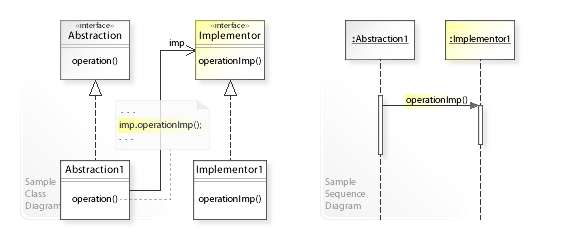
\includegraphics[scale=0.6]{bridge-uml.jpg}
    \end{figure}
  \end{frame}

  \begin{frame}{Diagramas de Sequencia e Classe UML}
No diagrama de classe UML acima, uma abstração (Abstraction) não é implementada como normalmente em uma hierarquia de herança. Em vez disso, há uma hierarquia para uma abstração (Abstraction) e uma hierarquia separada para sua implementação (Implementor), o que faz destas duas independentes uma da outra. A interface Abstraction ( operation() ) é implementada pelos termos de (delegado para) a interface Implementor( imp.operationImp() ).
  \end{frame}

  \begin{frame}{Diagramas de Sequencia e Classe UML}
O diagrama de sequência UML mostra as interações em tempo de execução: o objeto Abstraction1 delega a implementação para o objeto Implementor1 ( chamando o operationImp() em Implementor1 ), o que realiza a operação e retorna para Abstraction1.
  \end{frame}

  \section{Exemplo}
  \begin{frame}{Exemplo}
O código a seguir (feito em Java SE 6) ilustra a implementação de uma 'forma' para desenho.
  \end{frame}

  \begin{frame}[fragile]
    \begin{lstlisting}{Java}
// Implementador

interface DesenhoAPI {
    public void desenharCirculo(final double x, final double y, final double radius);
}
    \end{lstlisting}
  \end{frame}

  \begin{frame}[fragile]
    \begin{lstlisting}{Java}
// Implementador Concreto 1

class DesenhoAPI1 implements DesenhoAPI {
    public void desenharCirculo(final double x, final double y, final double radius) {
        System.out.printf("API1.circulo em %f:%f - radius %f\n", x, y, radius);
    }
}
    \end{lstlisting}
  \end{frame}
  
  \begin{frame}[fragile]
  \begin{lstlisting}{Java}
// Implementador Concreto 2

class DesenhoAPI2 implements DesenhoAPI {
    public void desenharCirculo(final double x, final double y, final double radius) {
        System.out.printf("API2.circulo em %f:%f - radius %f\n", x, y, radius);
    }
}
    \end{lstlisting}
  \end{frame}

  \begin{frame}[fragile]
  \begin{lstlisting}{Java}
// Abstracao

abstract class Forma {
    protected DesenhoAPI desenhoAPI;
    
    protected Forma(final DesenhoAPI desenhoAPI) {
        this.desenhoAPI = desenhoAPI;
    } 

    public abstract void desenhar(); // baixo nivel
    public abstract void alterarTamanhoPorPorcentagem(final double pct); // alto nivel
}
    \end{lstlisting}
  \end{frame}

  \begin{frame}[fragile]
  \begin{lstlisting}{Java}
// Abstracao Refinada

class FormaCirculo extends Forma() {
    private double x, y, radius;

    public FormaCirculo(final double x, final double y, final double radius, final DesenhoAPI desenhoAPI) {
        super(desenhoAPI);
        this.x = x;
        this.y = y;
        this.radius = radius;
    }
    \end{lstlisting}
  \end{frame}

  \begin{frame}[fragile]
  \begin{lstlisting}{Java}
// implementacao de baixo nivel (especifico da implementacao)
    public void desenhar() {
        desenhoAPI.desenharCirculo(x, y, radius);
    }

    // implementacao de alto nivel (especifico da abstracao)
    public void alterarTamanhoPorPorcentagem(final double pct) {
        radius *= (1.0 + pct/100.0);
    }
}
    \end{lstlisting}
  \end{frame}

  \begin{frame}[fragile]
  \begin{lstlisting}{Java}
// Cliente

class PadraoBridge {
    public static void main(final String[] args) {
        Forma[] formas = new Forma[] {
            new FormaCirculo(1, 2, 3, new DesenhoAPI1()),
            new FormaCirculo(5, 7, 11, new DesenhoAPI2())
        };

        for (Forma forma: formas) {
            forma.alterarTamanhoPorPorcentagem(2.5);
            forma.desenhar();
        }
    }
}
    \end{lstlisting}
  \end{frame}
  
\section{Conclusão}  
  
\begin{frame}{Conclusão}
	Tendo em vista o exemplo anterior, temos um problema facilmente tratado pelo padrão Bridge resolvido. 
	
	A interface DesenhoAPI é o topo da hierarquia da parte de implementação do programa, enquanto que a classe abstrata Forma é o topo da parte abstrata, perceba que uma composição de baixo nível do sistema utiliza a interface DesenhoAPI para implementar a função de desenho, enquanto que a composição de alto nível permite alterar o tamanho do desenho ainda na parte abstrata, separando esta da implementação do resto do programa.
\end{frame}

\begin{frame}{Conclusão}
	Separando a implementação de alto nível podemos evitar a repetição de código, enquanto que separado a implementação de baixo nível nos permite reaproveitar partes de código enquanto que mantém o sistema desacoplado, estas funcionalidades simples do padrão de projeto facilitam o trabalho do programador que o desenvolve, enquanto que ajuda outros desenvolvedores a entenderem partes do projeto sem ter conhecimento de todo o funcionamento do programa.
\end{frame}

\begin{frame}{Referências}

- Gamma, E, Helm, R, Johnson, R, Vlissides, J: Design Patterns, page 151. Addison-Wesley, 1995

- Erich Gamma, Richard Helm, Ralph Johnson, John Vlissides (1994). Design Patterns: Elements of Reusable Object-Oriented Software. Addison Wesley. pp. 151ff. ISBN 0-201-63361-2.

- "The Bridge design pattern - Problem, Solution, and Applicability". w3sDesign.com. Retrieved 2017-08-12.

- "The Bridge design pattern - Structure and Collaboration". w3sDesign.com. Retrieved 2017-08-12.

- Bridge Pattern - Wikipedia

\end{frame}

\end{document}
